\documentclass{article}
\usepackage{amsmath}
\usepackage{caption}
\usepackage{multirow}
\usepackage{wrapfig}
\usepackage[T2A]{fontenc}
\usepackage[english,russian]{babel}
\usepackage{graphicx}
\usepackage{subfig}
\usepackage[a4paper,top=2cm,bottom=2cm,left=1.5cm,right=1.5cm,marginparwidth=1.75cm]{geometry}
\usepackage{indentfirst}
\usepackage{physics}
\usepackage{mathtools}
\usepackage{extarrows}
\usepackage{nicefrac}
\usepackage[colorlinks=true, allcolors=blue]{hyperref}

\newcommand{\x}{\text}
\newcommand{\ii}{\textit}
\newcommand{\bb}{\textbf}
\newcommand*\textfrac[2]{
  \frac{\text{#1}}{\text{#2}}
}

\date{}
\author{}
\title{Лaбораторная работа 2.3.1 \\ Получение и измерение вакуума при турбомолекулярной откачке}

\begin{document}
\maketitle

\section*{Аннотация}


\paragraph{Цель работы:} 1) измерение объемов форвакуумной и высоковакуумной частей установки; 2) определение скорости откачки системы в стационарном режиме, а также по ухудшению и улучшению вакуума.
\paragraph{В работе используются:} вакуумная установка с манометрами: масляным, термопарным и ионизационным.



\section*{Теоретические сведения}

В физике \textbf{вакуумом} называется состояние газа, при котором характерная длина свободного пробега молекул в газе $\lambda$ сравнима по порядку величины с характерным линейным размером сосуда $d$, в котором газ находится.
В технике вакуумом называют состояние газа, при котором его давление меньше атмосферного ($P < P_\text{атм}$), различая три основных типа:
\begin{enumerate}
    \item Низкий, когда $\lambda < d$
    \item Срединй, когда $\lambda \sim d$
    \item Высокий, когда $\lambda > d$
\end{enumerate}

\begin{figure}[h!]
    \centering
    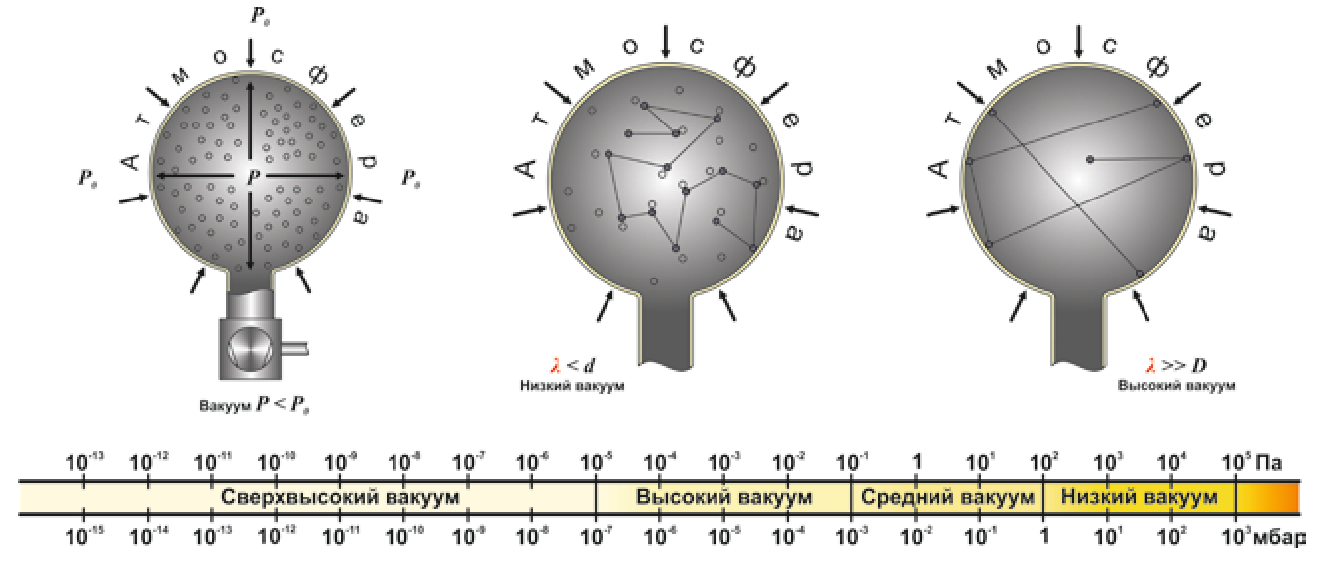
\includegraphics[width=\textwidth]{pic1.png}
\end{figure}

% \subsection*{Некоторые понятия для работы с вакуумной техникой}

% \textbf{Предельное остаточное давление (предельный вакуум)} -- наименьшее давление газа, которое формируется в процессе откачки в рассматриваемом сечении вакуумпровода (рассматриваемой точек вакуумной системы).

% \textbf{Наибольшее выпускное давление} -- максимально допустимое давление газа на входе насоса.

% \textbf{Быстрота откачивающего действия (скорость откачки) вакуумной системы} S$[L^3 T^{-1}]$ -- объём газа, проходящий через рассматриваемое сечение вакуумпровода в единицу времени при текущем давлении в данном сечении:
% \begin{equation}\nonumber
%     S = \frac{dV}{dt}
% \end{equation}

% \bb{Быстродействие} насоса определяется как:
% \begin{equation}\label{eq1}
%     \boxed{S_\text{н} = \frac{d V_\text{н}}{dt}}
% \end{equation}
% а \bb{эффективная скорость откачки камеры} $S_0$ как:
% \begin{equation}
%     \boxed{S_\text{о} = \frac{d V_\text{о}}{dt}}
% \end{equation}

% \bb{Падение давления} вдоль вакуумпровода $\Delta P = P_1 - P_2$ определяется его пропускной способностью (проводимостью) $U \; [L^3T^{-1}] $:
% \begin{equation}
%     U = \frac{Q}{P_1 - P_2}
% \end{equation}
% где $Q \; [L^2 M T^{-3}] $ -- поток газа через вакуумпровод с соответствующими давлениями на концах.

% Величина $Z$, обратная проводимости, называется \bb{импендансом} вакуумпровода.

% В общем случае эти величины зависят от времени, но в конце откачки устанавливается квазистационарный режим, при котором поток газа становится практически постоянным и равным потоку газа, потступающему через течи. Для стационарного режима можно записать:
% \begin{equation}\label{eq4}
%     P_1 S_\x{о} = P S = P_2 S_\x{н} = Q
% \end{equation}

% Из уравнений (\ref{eq1}--\ref{eq4}) можно получить \bb{основное уравнение вакуумной техники}:
% \begin{equation}\label{eq5}
%     \boxed{\frac{1}{S_\x{о}} = \frac{1}{S_\x{н}} + \frac{1}{U}}
% \end{equation}

% Количественной характеристикой течи является \bb{натекание}
% \begin{equation}
%     \boxed{Q_\x{н} = V \frac{P_\x{к} - P_\x{н}}{\Delta t}}
% \end{equation}
% где $V$ -- замкнутый исследуемый объём; $P_\x{н}$, $P_\x{к}$ -- начальное и конечное давление в объёме; $\Delta t$ -- время между измерениями давления.

% На пропускную способность вакуумпровода существенно влияет режим течения газа, который характерзуется \bb{числом Кнудсена}:
% \begin{equation}
%     \boxed{\x{Kn} = \frac{\lambda}{d}}
% \end{equation}

% Данная величина характеризует степень разреженности газового потока:
% \begin{enumerate}
%     \item Если $\x{Kn} \ll 1$ (Гидродинамический режим течения), различают \ii{ламинарные} -- когда молекулы газа движутся по параллельным траекториям со схожими скоростями, и \ii{турулентные} -- когда молекулы движутся хаотически со скоростями, подвергающимися случайным изменениям, потоки.
%     \item Если $\x{Kn} \gg 1$ (молекулярный (кнудсеновский) режим течения), течение газа сводится к незаисимому движению отдельных молекул по прямым линиям.
%     \item Если $\x{Kn} \sim 1$, в системе могут существовать все описанные выше виды течения.
% \end{enumerate}

% \subsection*{Проводимость отверстия в стенке}

% Для кнудсеновского режима, проведя некоторые оценки, можно получить формулу проводимости отверстия:
% \begin{equation}
%     \boxed{U_\x{отв} = \frac{1}{4} \pi R^2 \sqrt{\frac{8 k T}{\pi m}} \sim R^2 \sqrt{\frac{T}{m}} }
% \end{equation}
% где $R$ -- радиус отверсти, $m$ -- масса молекулы газа, $T$ -- температура газа.

% \subsection*{Проводимость длинного трубопровода}

% Проводимость длинного труопровода ($L \gg R$) в \bb{гидродинамическом режиме} может быть получена из формулы Пуазейля:
% \begin{equation}
%     \boxed{U_\x{тр} = \frac{Q}{P_2 - P_1} = P \frac{\pi R^4}{8 \eta L} \sim \frac{R^4}{L}\frac{P}{\sqrt{T m}}}
% \end{equation}
% где $P$ -- давление в рассматриваемом сечении трубы (среднее по длине $ P = (P_1 + P_2)/2) $, $\eta$ -- вязкость газа, $L$ -- длина трубопровода, $R$ -- его радиус.

% А в \bb{молекулярном режиме} из формулы Кнудсена:
% \begin{equation}\label{eq6}
%     \boxed{U_\x{тр} = \frac{Q}{P_2 - P_1} = \frac{4}{3} \frac{R^3}{L} \sqrt{\frac{2 \pi k T}{m}} \sim \frac{R^3}{L}\sqrt{\frac{T}{m}}}
% \end{equation}

% Для промежуточного случая производится интерполяция.

% \begin{equation}
%     \boxed{\frac{d(PV)}{dt}\equiv Q = \frac{4}{3} r^3 \sqrt{\frac{2 \pi R T}{\mu}}\frac{P_2 - P_1}{l}}
% \end{equation}

% При последовательном соединении разных вакуумпроводов, их импендансы суммируются:
% \begin{equation}
%     \boxed{U_\Sigma = \frac{1}{Z_\Sigma} = 1/\sum\limits_{(i)}{Z_i}}
% \end{equation}

% Из полученных соотношений можно сделать вывод: для эффективной откачки следует выбирать вакуумпроводы как можно шире и как можно короче; также не имеет смысла выбирать насос с производительностью $S_\x{н} \gg U_\Sigma$, поскольку тогда скорость откачки будет определяться, в основном проводимостью вакуумпровода.

% \subsection*{Время откачки}

% Положим, что за прмежуток времени $d t$ давление в откачиваемом объёме $V_\x{о}$ снижается на $d P_1$. Тогда за промежуток времени $dt$ количество газа, поступающего в трубку равно $S_\x{о} P_1 dt$, а эта же убыль газа в объёме равна $V_\x{о} dP_1$, следовательно:
% \begin{equation}\label{eq16}
%     S_\x{о} P_1 dt = - V_\x{о} dP_1
% \end{equation}
% \begin{equation}
%     dt = - \frac{V_\x{о}}{S_\x{о}} \frac{dP_1}{P_1}
% \end{equation}
% C учётом (\ref{eq5}), получим:
% \begin{equation}
%     dt = - V_\x{о} \left(\frac{1}{S_\x{н}} + \frac{1}{U}\right)\frac{dP_1}{P_1}
% \end{equation}
% При $S_\x{о} = const$, решение уравнения (\ref{eq16}) имеет вид:
% \begin{equation}\label{that_one}
%     \boxed{P(t) = P_1 \exp\left(-\frac{S_\x{о}}{V_\x{о}}t\right)+P_\x{пр}}
% \end{equation}
% \bb{Постоянная времени откачки} $\tau = V_\x{о}/S_\x{о}$ является мерой эффективности откачной системы.

\section*{Экспериментальная установка}


\bb{Установка состоит из} форвакуумного баллона (ФБ), высоковакуумного диффузионного насоса (ВН), высоковакуумного баллона (ВБ), масляного (М) и ионизационного (И) манометров, термопарных манометров (M$_1$ и М$_2$), форвакуумного насоса (ФН) и соединительных кранов К$_1$, К$_2$, $\ldots$ , К$_6$. Кроме того, в состав установки входят: вариатор (автотрансформатор с регулируемым выходным напряжением), или реостат и амперметр для регулирования тока нагревателя диффузионного насоса.

\newpage

\begin{figure}[h!]
    \centering
    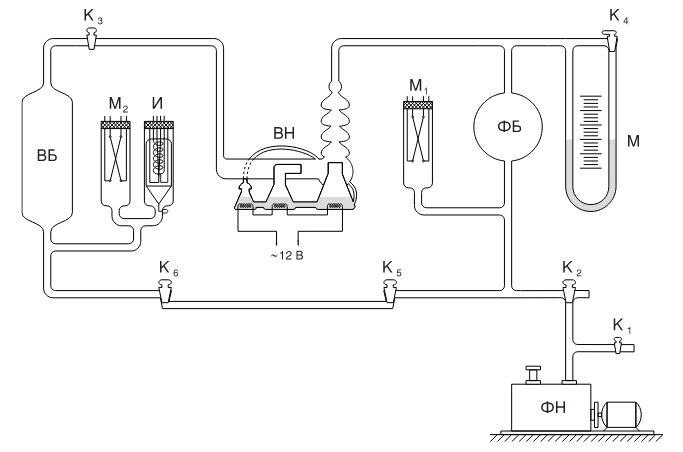
\includegraphics[width = 0.6\textwidth]{Screenshot from 2023-02-16 23-39-12.png}
    \caption{Схема экспериментальной установки}
    \label{pic1}
\end{figure}

\bb{Назначение кранов}:
\begin{enumerate}
    \item Используется для заполнения форвакуумного насоса и вакуумной установки атмосферным воздухом
    \item Используется для соединения форвакуумного насоса с установкой или атмосферой
    \item Отделяет высоковакуумную часть установки от форвакуумной
    \item Соединяет между собой колена масляного манометра
    \item и \; 6. стоят по концам капилляра и соединяют его с форвакуумной и высоковакуумной частями установки.
\end{enumerate}

\bb{Форвакуумный насос}. В цилинадгрической полости корпуса расположен эксцентрично ротор так, что он посотянно соприкасается своей верхней частью с корпусом. В диаметральный разрез ротора вставлены две пластины, раздвигаемые пружиной и плотно прижимаемые к поверхности полости. Они разделяют объём между ротором и корпусом на две части. В процессе вращения ротора в одну из частей откачиваемый газ поступает, а из другой выталкивается.

\begin{figure}[h!]
    \centering
    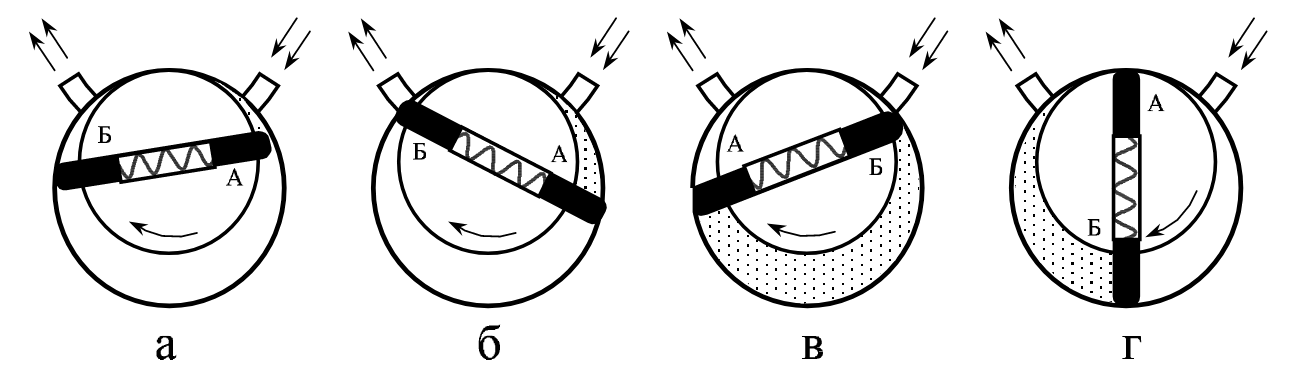
\includegraphics[width=0.7\textwidth]{Screenshot from 2023-02-21 13-13-09.png}
    \caption{Принцип действия форвакуумного насоса}
    \label{pic2}
\end{figure}

\bb{Диффузионный насос}. Откачивающее действие основано на внедрении молекул разреженного воздуха в струю паров масла. Попавшие в струю молекулы увлекаются ею и уже не возвращаются назад. На прежнем их месте образуется пустота, которая немедленно заполняется следующими порциями газа, увеличивая степень разрежения газа в окрестности струи и оказывая таким образом сильне откачивающее воздействие на весь газ в откачиваемом объёме. Скорость откачки диффузионных насосов в сотни и тысячи раз превосходит скорость откачки форвакуумных насосов.

Масло, налиотое в сосуд А, подогревается электической печкой. Пары масла поднимаются по трубе Б и вырываются из сопла В. Струя паров увлекает молекулы газа, которые поступают через трубку ВВ. Дальше смесь попадает в вертикальную трубу Г. Здесб масло осаждается на стенках трубы и маслообменников и стекает вниз, а оставшийся газ через трубу ФВ откачивается форвакуумным насосом.
\newpage

\begin{figure}[!h]
    \centering
    \subfloat[Схема работы диффузионного насоса]{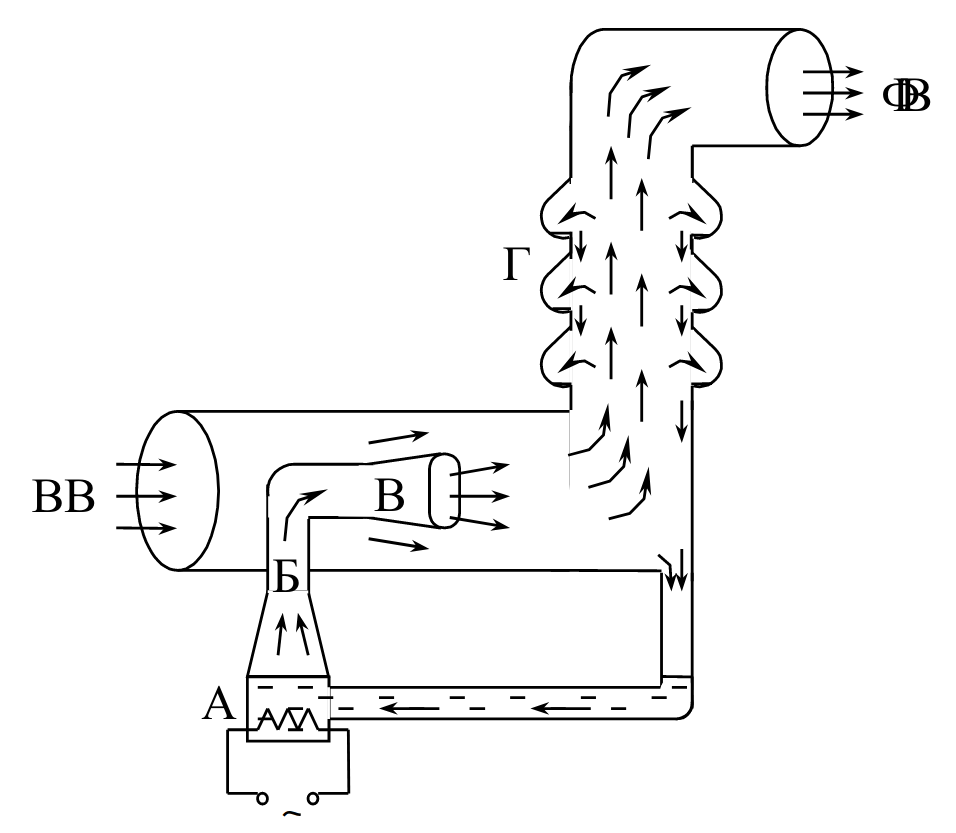
\includegraphics[width=0.5\textwidth]{Screenshot from 2023-02-21 13-44-11.png}\label{pic6}}
    \hfill
    \subfloat[Схема лампы]{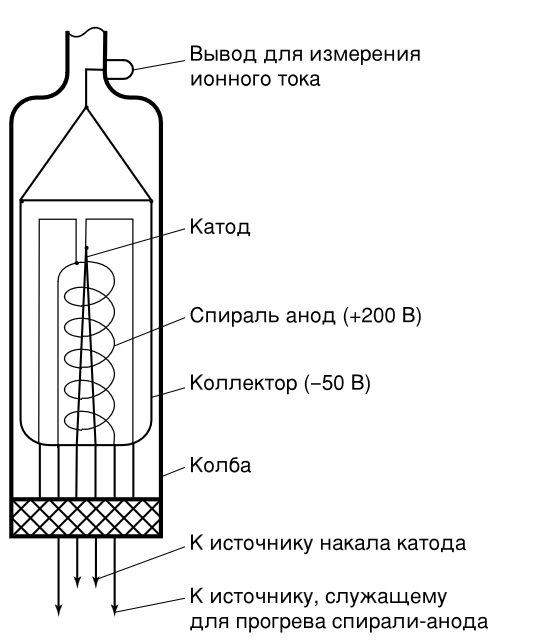
\includegraphics[width=0.3\textwidth]{Screenshot from 2023-02-22 19-56-21.png}\label{pic3}}
\end{figure}

В нашей установке диффузионый насос имеет две ступени и соответственно два сопла. Первая ступень обогащается с помощью второй печи и плотность её струи выше, поэтому она начинает откачивать при более высоком давлении в форвакуумной части установки. Во второй ступени плотность струи меньше и она начинает откачивать при меньшем давлении.

\bb{Масляный манометр} представляет собой U-образную трубку, до половины наполненную вязким маслом, обладающим весьма низким давлением насыщенных паров. Так как плотность масла мала, при помощи манометра можно измерить только небольшие разности давлений.

\bb{Ионизационный манометр} представляет собой трехэлектродную лампу (\ref{pic6}). Электроны испускаются накаленным катодом и увлекаются электрическим полем к аноду, имеющему вид редкой спирали. Далее они замедляются полем коллетора и возвращаются к катоду. На своём пути электроны ионизируют молекулы газа. Ионы притягиваются полем коллектора.

\subsection*{Процесс откачки}
Опишем процесс откачки математически:
Пусть W --- объем газа, удаляемого из сосуда при данном давлении за единицу времени, $Q_i$ для различных значений i обозначим различные притоки газа в сосуд (в единицах PV), такие как течи извне $Q_\text{и}$, десорбция с поверхностей внутри сосуда $Q_\text{д}$, обратный ток через насос $Q_\text{н}$. Тогда, приравнивая убыль газа из сосуда (с точностью до $RT/\mu$) в единицу времени $-VdP$ и сумму перечисленных токов? имеем:
\begin{equation}\label{eq11}
    -VdP = (PW - \sum_i Q_i)dt
\end{equation}
При достижении предельного вакуума устанавливается давление $P_{\text{пр}}$, и $dP = 0$. Тогда
\begin{equation}\label{eq22}
    W = ( \sum_i Q_i )/P_{\text{пр}}
\end{equation}
Поскольку обычно $Q_\text{и}$ постоянно, а $Q_\text{н}$ и $Q_\text{д}$ слабо зависят от времени, также считая постоянной W, можем проинтегрировать (\ref{eq11}) и получить:
\begin{equation}\label{that_one}
    P - P_{\text{пр}} = (P_0 - P_{\text{пр}})\exp(-\frac{W}{V}t)
\end{equation}
Полная скорость откачки $W$, собственная скорость откачки насоса $W_{\text{н}}$ и проводимости элементов системы $C_1, C_2,...$ соотносятся согласно формуле (\ref{eq44}), и это учтено в конструкции установки.
\begin{equation}\label{eq44}
    \frac{1}{W} = \frac{1}{W_\x{н}} + \frac{1}{C_1} + \frac{1}{C_2} + \ldots
\end{equation}

\subsection*{Течение газа через трубу}
Характер течения газа существенно зависит от соотношения между размерами системы и длиной свободного пробега молекул. При атмосферном и форвакуумном давлениях  длина свободного пробега меньше диаметра трубок, и течение газа определяется его вязкостью, т.е. взаимодействием молекул. При высоком вакууме течение существеннее определяется взаимодействием со стенками \\
Для количества газа, протекающего через трубу длины $l$ и радиуса $r$ в условиях высокого вакуума, справедлива формула:
\begin{equation}\label{eq55}
    \frac{d(PV)}{dt} = \frac{4}{3}r^3\sqrt{\frac{2\pi RT}{\mu}}\frac{P_2 - P_1}{l}
\end{equation}
Если труба соединяет насос установку, то давлением $P_1$ у насоса можно пренебречь. Давление в сосуде $P = P_2$. Тогда имеем:
\begin{equation}\label{eq6}
    C_\text{тр} = \left(\frac{dV}{dt}\right)_\text{тр} = \frac{4r^3}{3l}\sqrt{\frac{2\pi RT}{\mu}}
\end{equation}
Для пропускной способности отверстий имеется формула
\begin{equation}
    C_\text{отв} = \left(\frac{dV}{dt}\right)_\text{отв} = S\frac{\bar{\upsilon}}{4}
\end{equation}
Для воздуха при комнатной температуре $\bar{\upsilon}/4 = 110~\text{м/с} = 11~\text{л/c}\cdot\text{см}^2$.

\section*{Результаты измерений и обработка данных}

\begin{table}[h!]\centering
    \begin{tabular}{llllllll}
        \hline
        \multicolumn{4}{|c|}{Эксперимент 1} & \multicolumn{4}{|c|}{Эксперимент 2}                                                                                                                                                                                   \\\hline
        \multicolumn{2}{|c|}{Улучшение}     & \multicolumn{2}{|c|}{Ухудшение}     & \multicolumn{2}{|c|}{Улучшение} & \multicolumn{2}{|c|}{Ухудшение}                                                                                                               \\\hline
        \multicolumn{1}{|l|}{0  }           & \multicolumn{1}{|l|}{87 }           & \multicolumn{1}{|l|}{10 }       & \multicolumn{1}{|l|}{4.2}       & \multicolumn{1}{|l|}{0 } & \multicolumn{1}{|l|}{63 } & \multicolumn{1}{|l|}{0 } & \multicolumn{1}{|l|}{4.2} \\\hline
        \multicolumn{1}{|l|}{2  }           & \multicolumn{1}{|l|}{80 }           & \multicolumn{1}{|l|}{20 }       & \multicolumn{1}{|l|}{6  }       & \multicolumn{1}{|l|}{2 } & \multicolumn{1}{|l|}{50 } & \multicolumn{1}{|l|}{10} & \multicolumn{1}{|l|}{6.4} \\\hline
        \multicolumn{1}{|l|}{4  }           & \multicolumn{1}{|l|}{63 }           & \multicolumn{1}{|l|}{30 }       & \multicolumn{1}{|l|}{9.8}       & \multicolumn{1}{|l|}{4 } & \multicolumn{1}{|l|}{31 } & \multicolumn{1}{|l|}{20} & \multicolumn{1}{|l|}{10}  \\\hline
        \multicolumn{1}{|l|}{6  }           & \multicolumn{1}{|l|}{43 }           & \multicolumn{1}{|l|}{40 }       & \multicolumn{1}{|l|}{13 }       & \multicolumn{1}{|l|}{6 } & \multicolumn{1}{|l|}{22 } & \multicolumn{1}{|l|}{30} & \multicolumn{1}{|l|}{14}  \\\hline
        \multicolumn{1}{|l|}{7  }           & \multicolumn{1}{|l|}{29 }           & \multicolumn{1}{|l|}{50 }       & \multicolumn{1}{|l|}{16 }       & \multicolumn{1}{|l|}{8 } & \multicolumn{1}{|l|}{16 } & \multicolumn{1}{|l|}{40} & \multicolumn{1}{|l|}{18}  \\\hline
        \multicolumn{1}{|l|}{10 }           & \multicolumn{1}{|l|}{20 }           & \multicolumn{1}{|l|}{60 }       & \multicolumn{1}{|l|}{20 }       & \multicolumn{1}{|l|}{10} & \multicolumn{1}{|l|}{13 } & \multicolumn{1}{|l|}{50} & \multicolumn{1}{|l|}{22}  \\\hline
        \multicolumn{1}{|l|}{12 }           & \multicolumn{1}{|l|}{15 }           & \multicolumn{1}{|l|}{70 }       & \multicolumn{1}{|l|}{23 }       & \multicolumn{1}{|l|}{12} & \multicolumn{1}{|l|}{9.4} & \multicolumn{1}{|l|}{60} & \multicolumn{1}{|l|}{26}  \\\hline
        \multicolumn{1}{|l|}{14 }           & \multicolumn{1}{|l|}{11 }           & \multicolumn{1}{|l|}{80 }       & \multicolumn{1}{|l|}{27 }       & \multicolumn{1}{|l|}{14} & \multicolumn{1}{|l|}{8.1} & \multicolumn{1}{|l|}{70} & \multicolumn{1}{|l|}{30}  \\\hline
        \multicolumn{1}{|l|}{16 }           & \multicolumn{1}{|l|}{9.2}           & \multicolumn{1}{|l|}{90 }       & \multicolumn{1}{|l|}{31 }       & \multicolumn{1}{|l|}{16} & \multicolumn{1}{|l|}{7  } & \multicolumn{1}{|l|}{80} & \multicolumn{1}{|l|}{34}  \\\hline
        \multicolumn{1}{|l|}{18 }           & \multicolumn{1}{|l|}{7.4}           & \multicolumn{1}{|l|}{100}       & \multicolumn{1}{|l|}{34 }       & \multicolumn{1}{|l|}{18} & \multicolumn{1}{|l|}{6.1} & \multicolumn{1}{|l|}{90} & \multicolumn{1}{|l|}{38}  \\\hline
        \multicolumn{1}{|l|}{20 }           & \multicolumn{1}{|l|}{6.6}           & \multicolumn{1}{|l|}{110}       & \multicolumn{1}{|l|}{37 }       & \multicolumn{1}{|l|}{20} & \multicolumn{1}{|l|}{5.7} &                          &                           \\\cline{1-6}
        \multicolumn{1}{|l|}{22 }           & \multicolumn{1}{|l|}{6.1}           & \multicolumn{1}{|l|}{120}       & \multicolumn{1}{|l|}{42 }       & \multicolumn{1}{|l|}{22} & \multicolumn{1}{|l|}{5.4} &                          &                           \\\cline{1-6}
        \multicolumn{1}{|l|}{24 }           & \multicolumn{1}{|l|}{5.7}           & \multicolumn{1}{|l|}{130}       & \multicolumn{1}{|l|}{46 }       & \multicolumn{1}{|l|}{24} & \multicolumn{1}{|l|}{5.1} &                          &                           \\\cline{1-6}
                                            &                                     & \multicolumn{1}{|l|}{140}       & \multicolumn{1}{|l|}{50 }       &                          &                           &                          &                           \\\cline{3-4}
                                            &                                     & \multicolumn{1}{|l|}{150}       & \multicolumn{1}{|l|}{54 }       &                          &                           &                          &                           \\\cline{3-4}
                                            &                                     & \multicolumn{1}{|l|}{160}       & \multicolumn{1}{|l|}{57 }       &                          &                           &                          &                           \\\cline{3-4}
                                            &                                     & \multicolumn{1}{|l|}{170}       & \multicolumn{1}{|l|}{61 }       &                          &                           &                          &                           \\\cline{3-4}
                                            &                                     & \multicolumn{1}{|l|}{180}       & \multicolumn{1}{|l|}{66 }       &                          &                           &                          &                           \\\cline{3-4}
    \end{tabular}
\end{table}


\subsection*{Построение графика и вычисление $W$ высоковакуумного насоса}

Мы получили резултаты давления $p$, подчиняющиеся формуле (\ref{that_one}). Для того, чтобы получить линейную зависимость, проведём следующие преобразования:

$$p \longrightarrow f(P(t)) = \ln(P-P_{\x{пр}}) - \ln(P_1) = -\frac{W}{V}t$$

В реальности точно опредлеить предельное давление невозможно, поэтому зависимость имеет более сложный вид:

$$ f(P(t)) = \ln(P+\Delta P) - \ln(P_1)$$
где $\Delta P$ -- разница измеренного предельного давления с <<идеальным>> для формулы.

\begin{equation}\label{f}
    f(t) = \ln\left[ P_1 \exp\left(-\frac{W}{V} t\right) + \Delta P \right] - \ln P_1
\end{equation}

% \begin{wrapfigure}[9]{r}{0.4\textwidth}
%     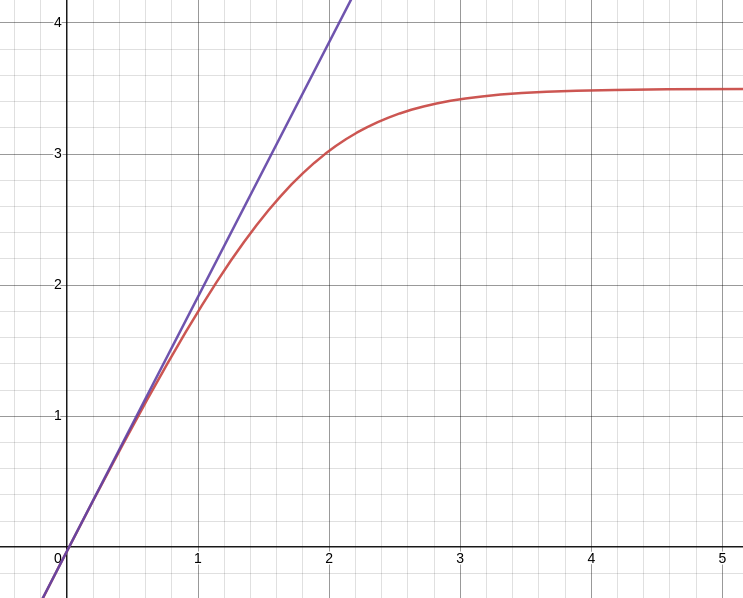
\includegraphics[width=0.4\textwidth]{Screenshot from 2023-03-01 22-42-54.png}
%     \caption{Приблизительный вид графика при малых $\Delta P$ и аппроксимация для малых $t$}
%     \label{approx}
% \end{wrapfigure}

Разложив по формуле Тейлора до $O(t)$ для маленьких $t$, получаем:

$$ f(t) \approx -\frac{P_1 (W/V)}{P_1 + \Delta P} t + \ln\left(\frac{P_1}{P_1 + \Delta P}\right)$$

Заметим, что при $\Delta P \ll P_1$ зависимость переходит в обычную пропорциональность $f(t) = (W/V)t$. В нашей работе $P_1/\Delta P \sim 10^2$, можно использовать это приближение.

Построим график для экспериментальных точек, применив эти преобразования (рис. \ref{wawa}).

\begin{figure}[!h]
    \centering
    \subfloat[Улучшение вакуума 1]{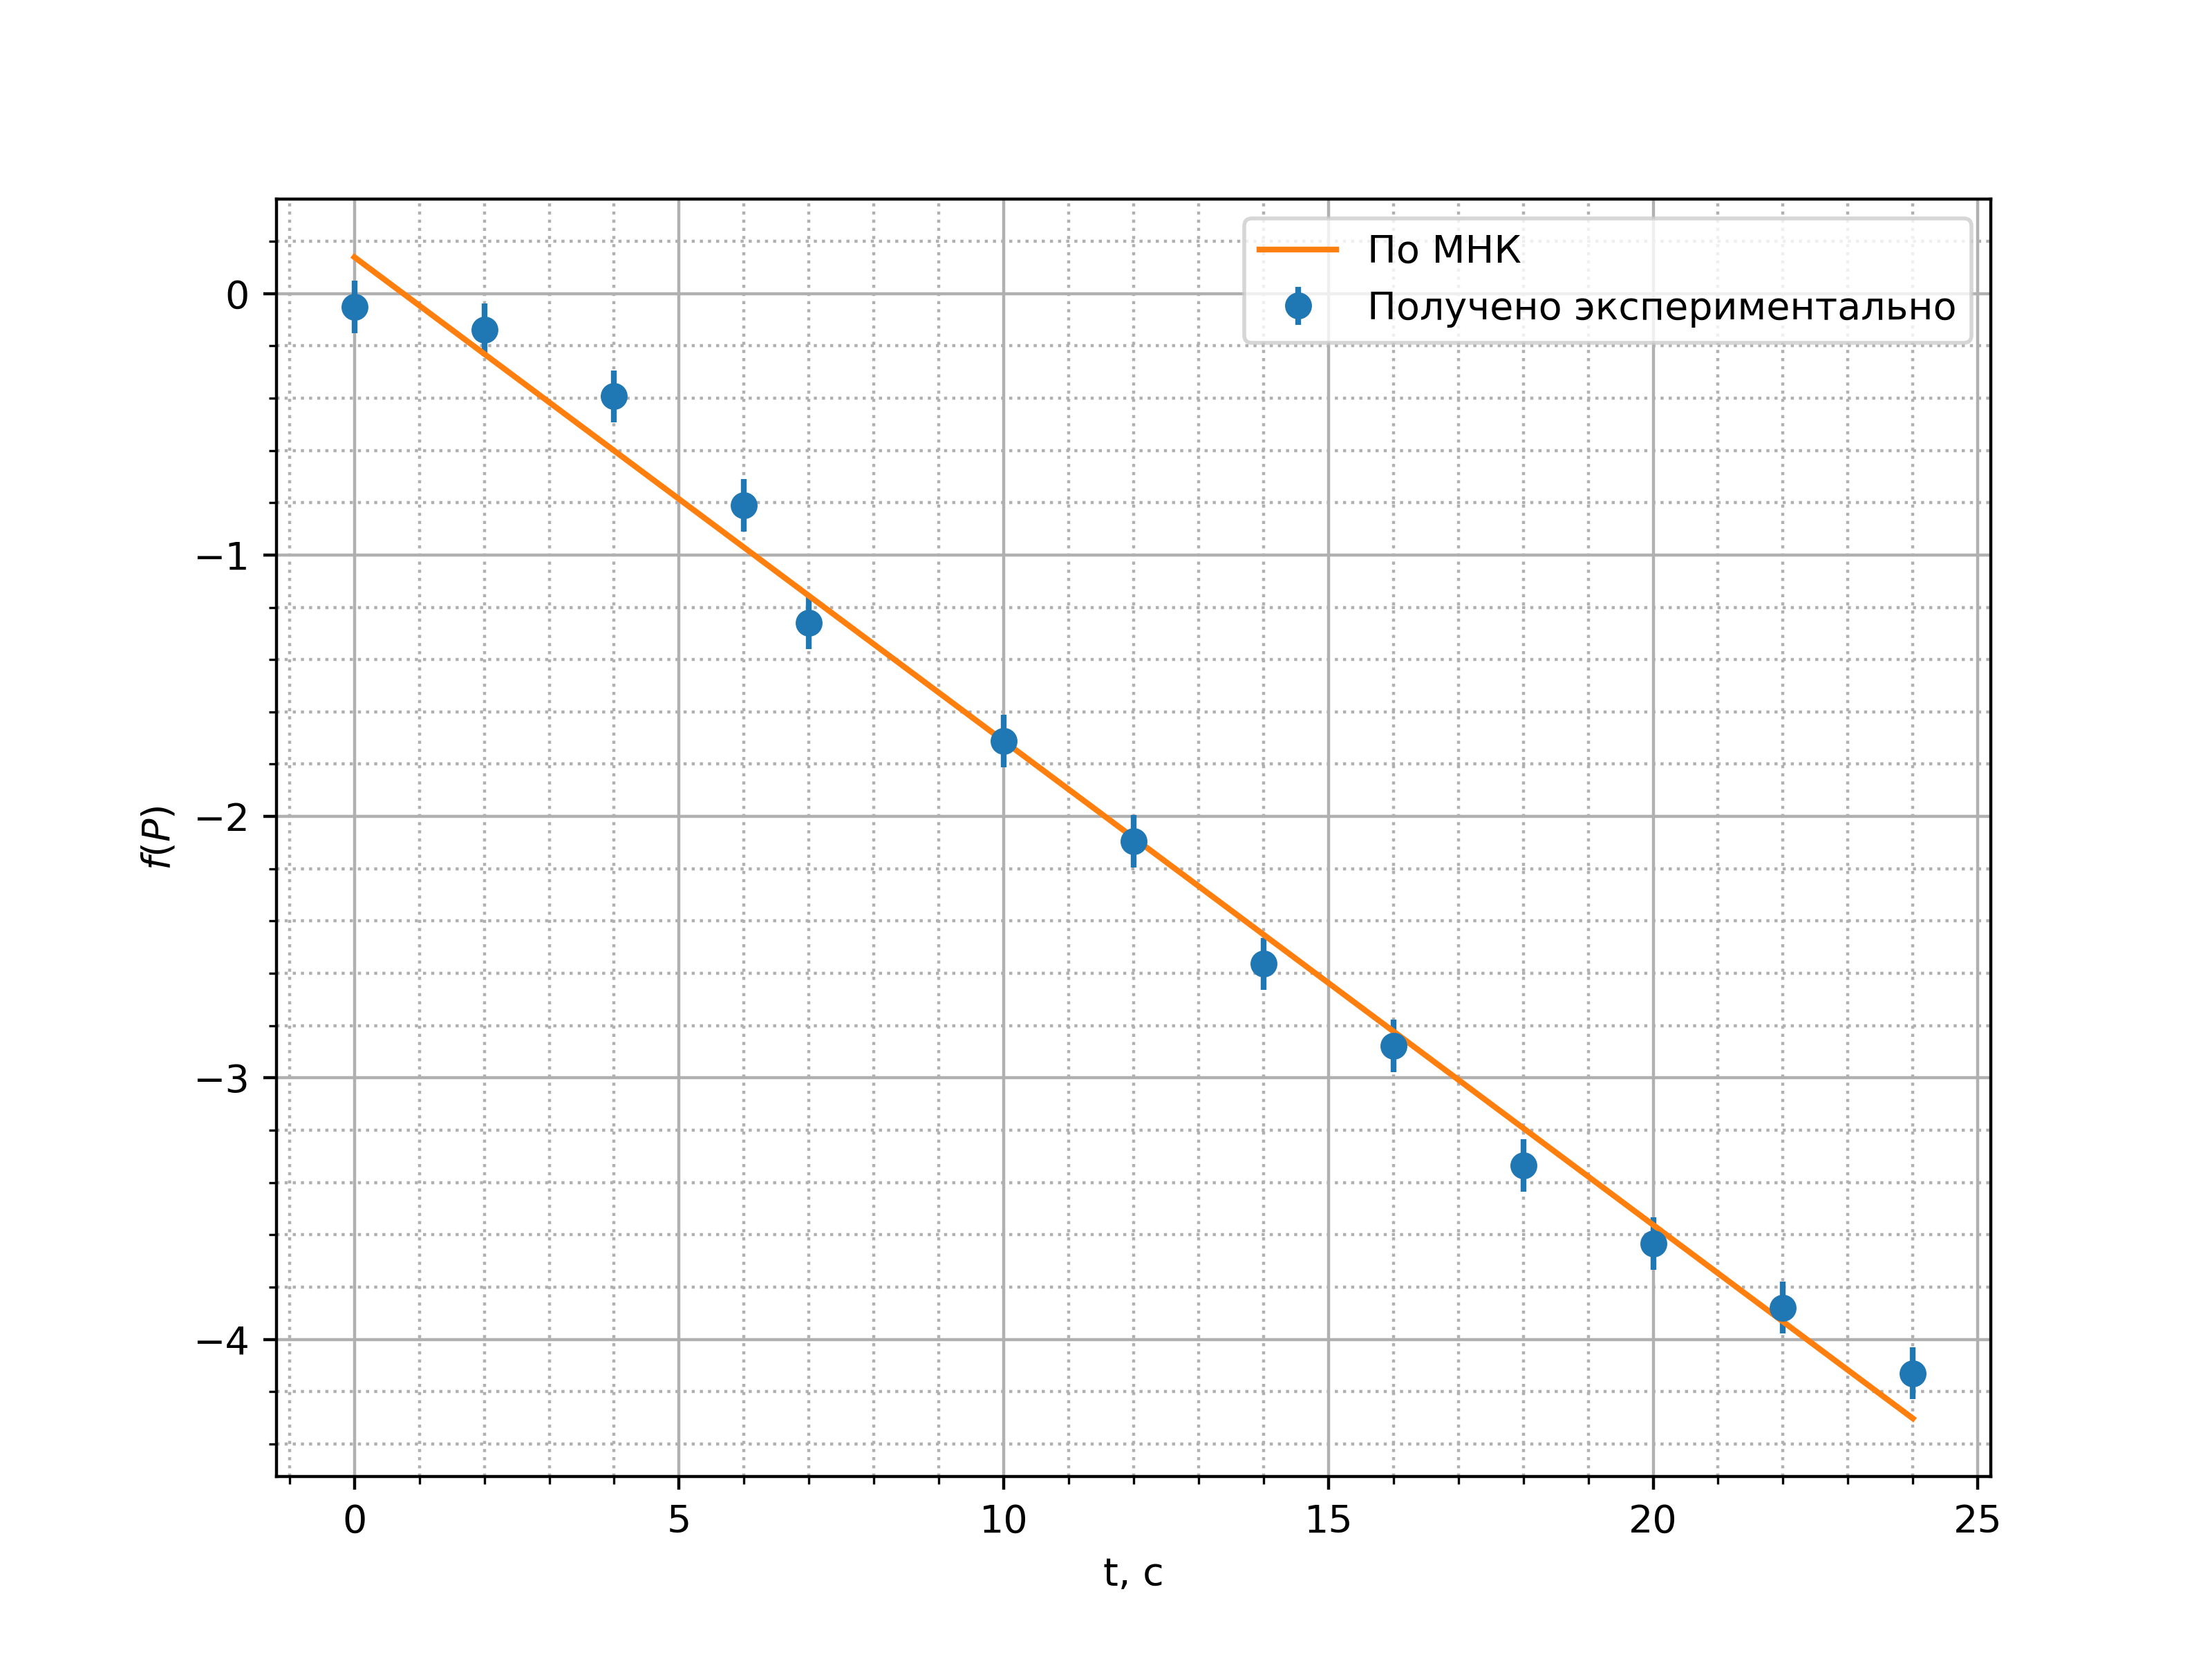
\includegraphics[width=0.5\textwidth]{diagram_v2.png}\label{fig:f1}}
    \hfill
    \subfloat[Улучшение вакуума 2]{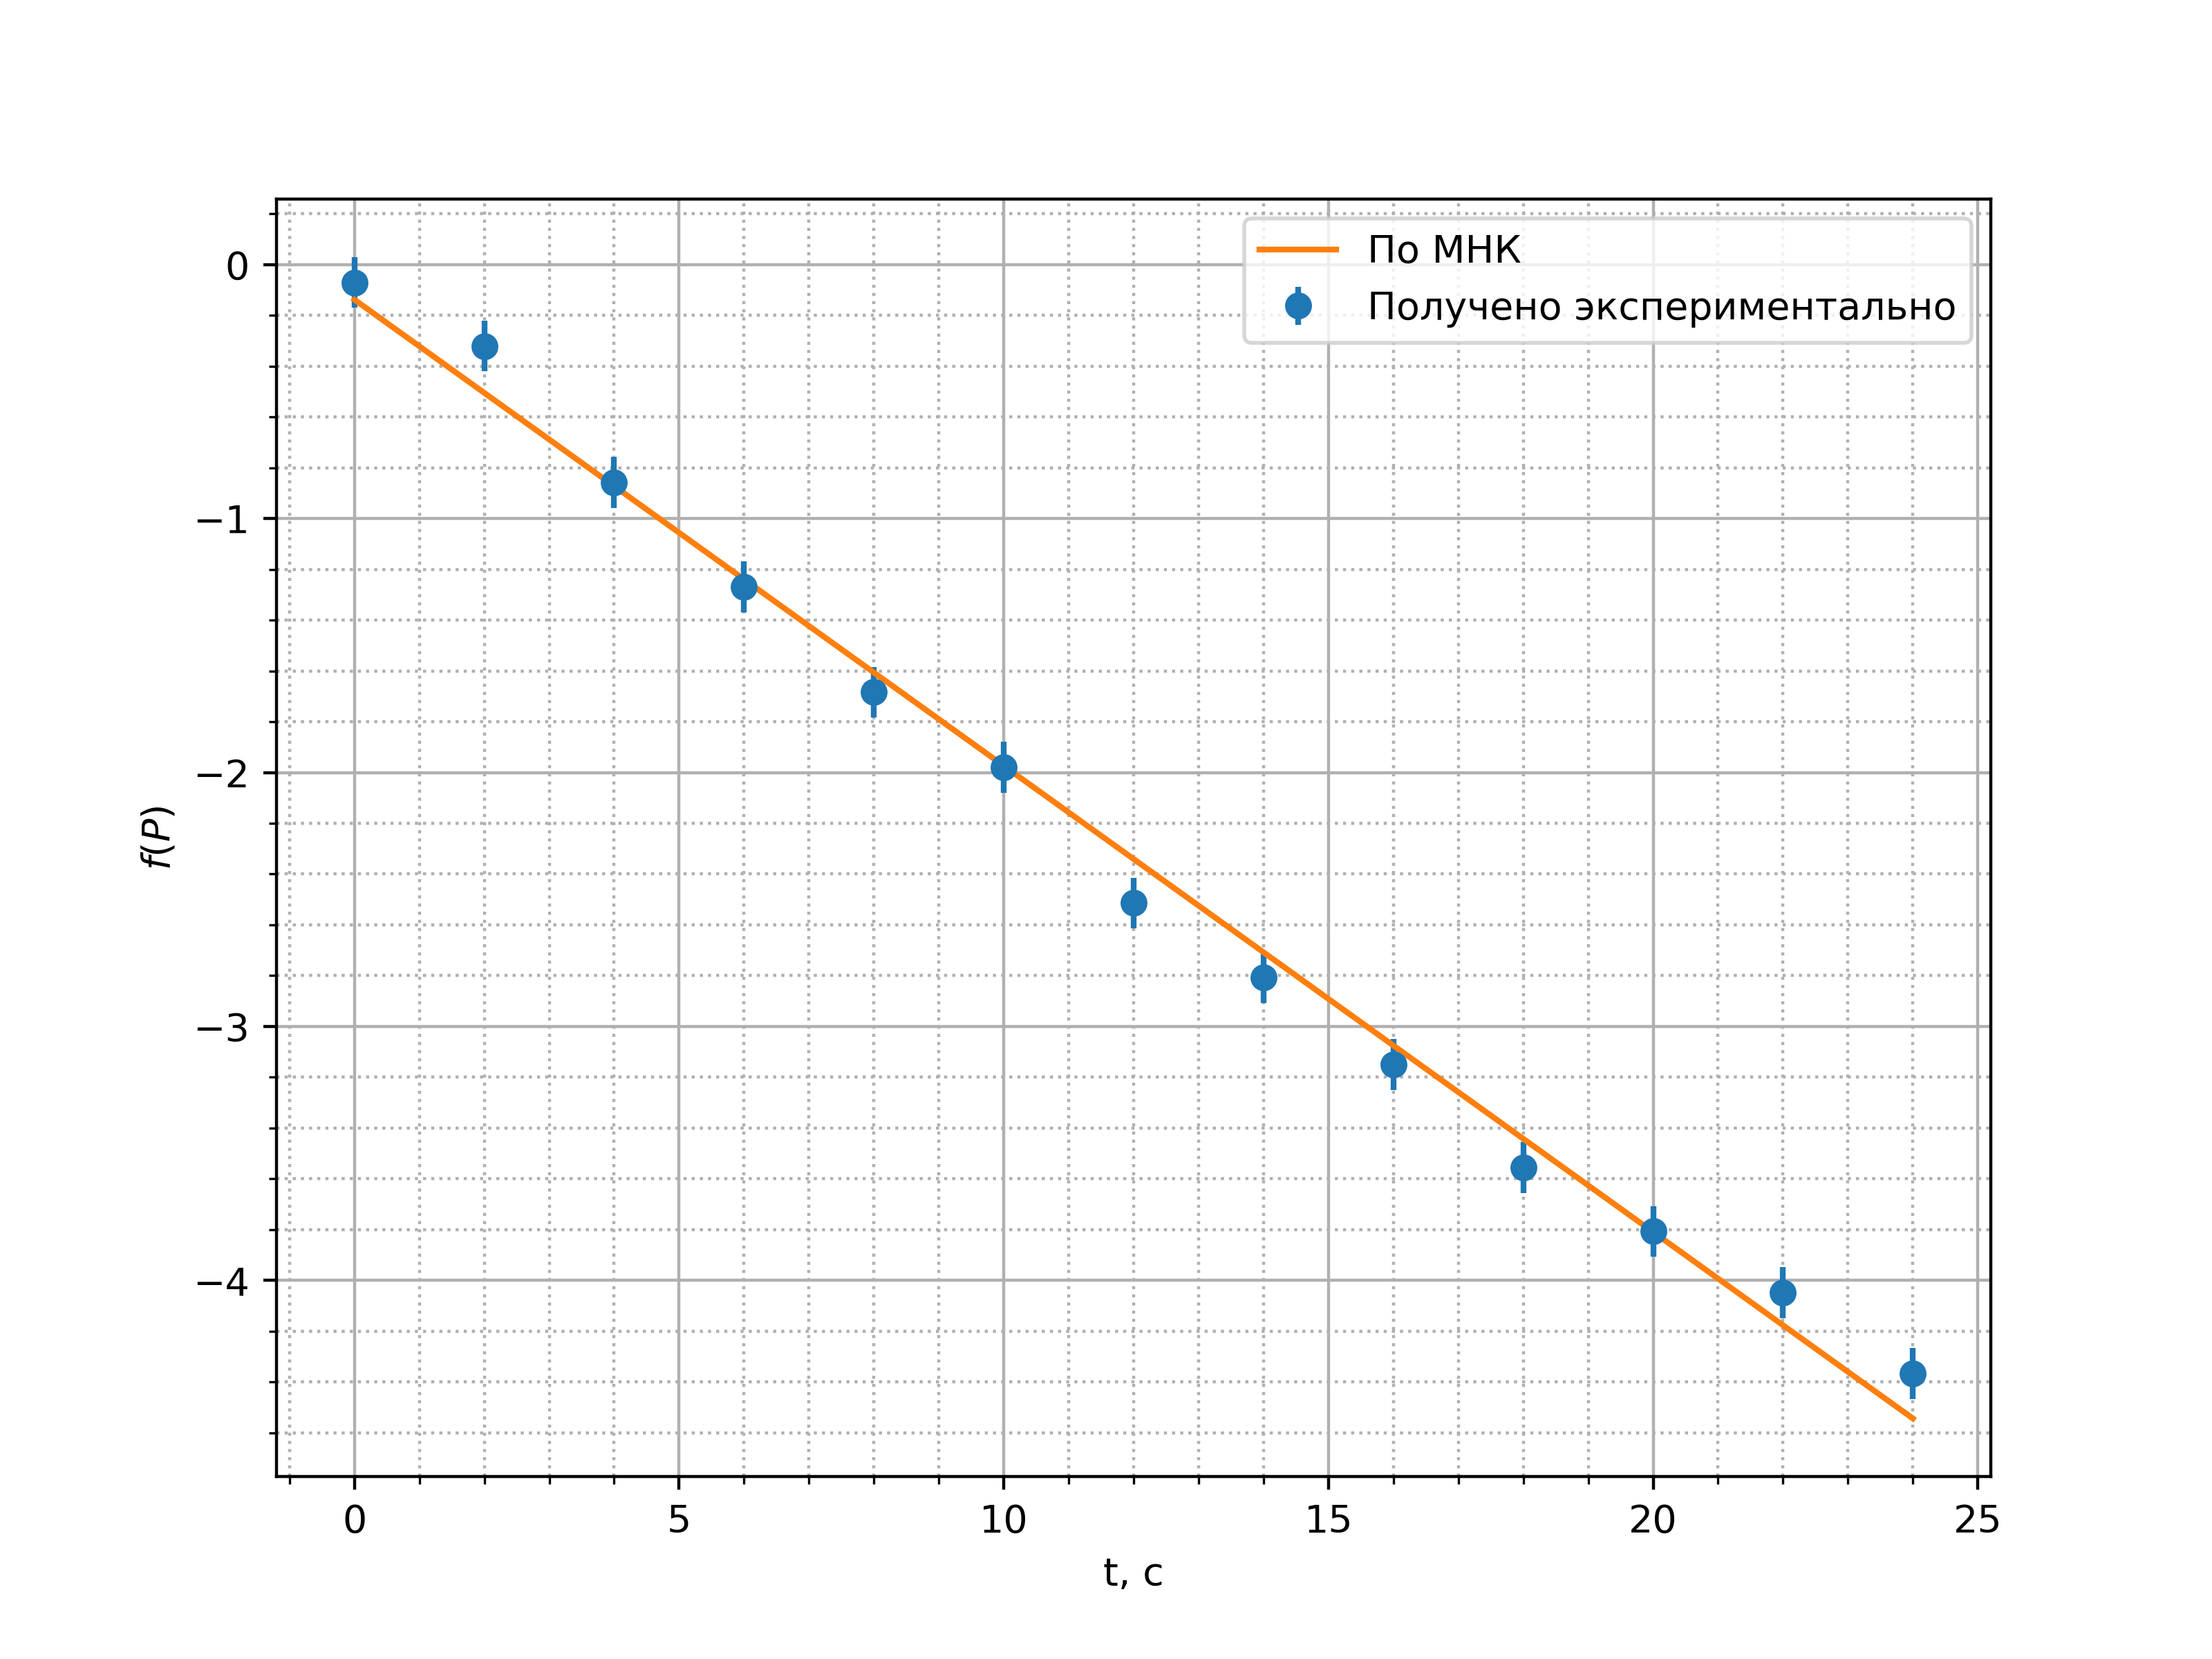
\includegraphics[width=0.5\textwidth]{diagram2_v2.png}\label{fig:f2}}
    \caption{Результаты экспериментов с применённой к ним $f(P)$}
    \label{wawa}
\end{figure}

\begin{table}[h!]
    \centering
    \begin{tabular}{|c|c|c|c|c|}
        \hline
          & $k, \; \x{с}^{-1}$ & $\sigma_k, \; \x{с}^{-1}$ & $V, \; \x{см}^{3}$    & $\sigma_V, \; \x{см}^3$ \\ \hline
        1 & -0.185             & 0.006                     & \multirow{2}{*}{1180} & \multirow{2}{*}{7}      \\ \cline{1-3}
        2 & -0.183             & 0.006                     &                       &                         \\ \hline
    \end{tabular}
\end{table}

$$\sigma_k = \sqrt{(\sigma_k^\x{случ})^2+(\sigma_k^\x{сист})^2}, \qquad \sigma_k^\x{сист} = k\sqrt{\varepsilon_V^2 + \varepsilon_P^2}$$

$$\sigma_{k_1} = \sqrt{0.003^2 + 0.005^2} = 0.006 \; \x{с}^{-1}, \qquad \sigma_{k_2} = \sqrt{0.003^3 + 0.005^2} = 0.006 \; \x{с}^{-1}$$

$$P_1 V_1 = P_2 V_2 \Rightarrow V_2 = \frac{P_1 V_1}{P_2} =  2122 \; \x{см}^{3}, \qquad P_2 V_2 = P_3 V_3 \Rightarrow V_3 = \frac{P_2 V_2}{P_3} = 3302  \; \x{см}^{3}, \qquad V_\x{вв} = V_3 - V_2 = 1180  \; \x{см}^{3}$$

$$\sigma_{V_2} = V_2 \sqrt{\left(\frac{\sigma_{P_2}}{P_2}\right)^2 + \left(\frac{\sigma_{P_1}}{P_1}\right)^2} \approx 4 \; \x{см}^3\; \qquad \sigma_{V_3} = V_3 \sqrt{\left(\frac{\sigma_{P_2}}{P_2}\right)^2 + \left(\frac{\sigma_{P_3}}{P_3}\right)^2 + \left(\frac{\sigma_{V_2}}{V_2}\right)^2} \approx 6 \; \x{см}^3$$

$$\sigma_{V_\x{вв}} = \sqrt{(\sigma_{V_3})^2 + (\sigma_{V_2})^2} = 7 \; \x{см}^3$$



Тогда получаем:
$$ k  = -\frac{W}{V}$$
$$ W = - kV = \frac{0.185 + 0.183}{2} \cdot 1183 \; \frac{\x{см}^3}{c} \approx 218.3 \; \frac{\x{см}^3}{c}, \qquad \sigma_W = W\sqrt{\varepsilon_k^2 + \varepsilon_V^2} = 218.3\sqrt{0.032^2 + 0.005^2} = 7.1 \; \frac{\x{см}^3}{c}$$
$$\boxed{W = 218.3\pm7.1 \; \frac{\x{см}^3}{c}} $$
\subsection*{Вычисление величины потока $Q_\x{н}$}

$$ V_\x{вв} dP = (Q_\x{д} + Q_\x{н})dt $$
$Q_\x{д} \ll Q_\x{н}$, поэтому можно записать:
$$\frac{dP}{dt} = \frac{Q_\x{н}}{V_\x{вв}}$$

$P$ от $t$ зависит линейно, поэтому значение ${dP}/{dt}$ можно найти с помощью метода наименьших квадратов.

\begin{figure}[!h]
    \centering
    \subfloat[Ухудшение вакуума 1]{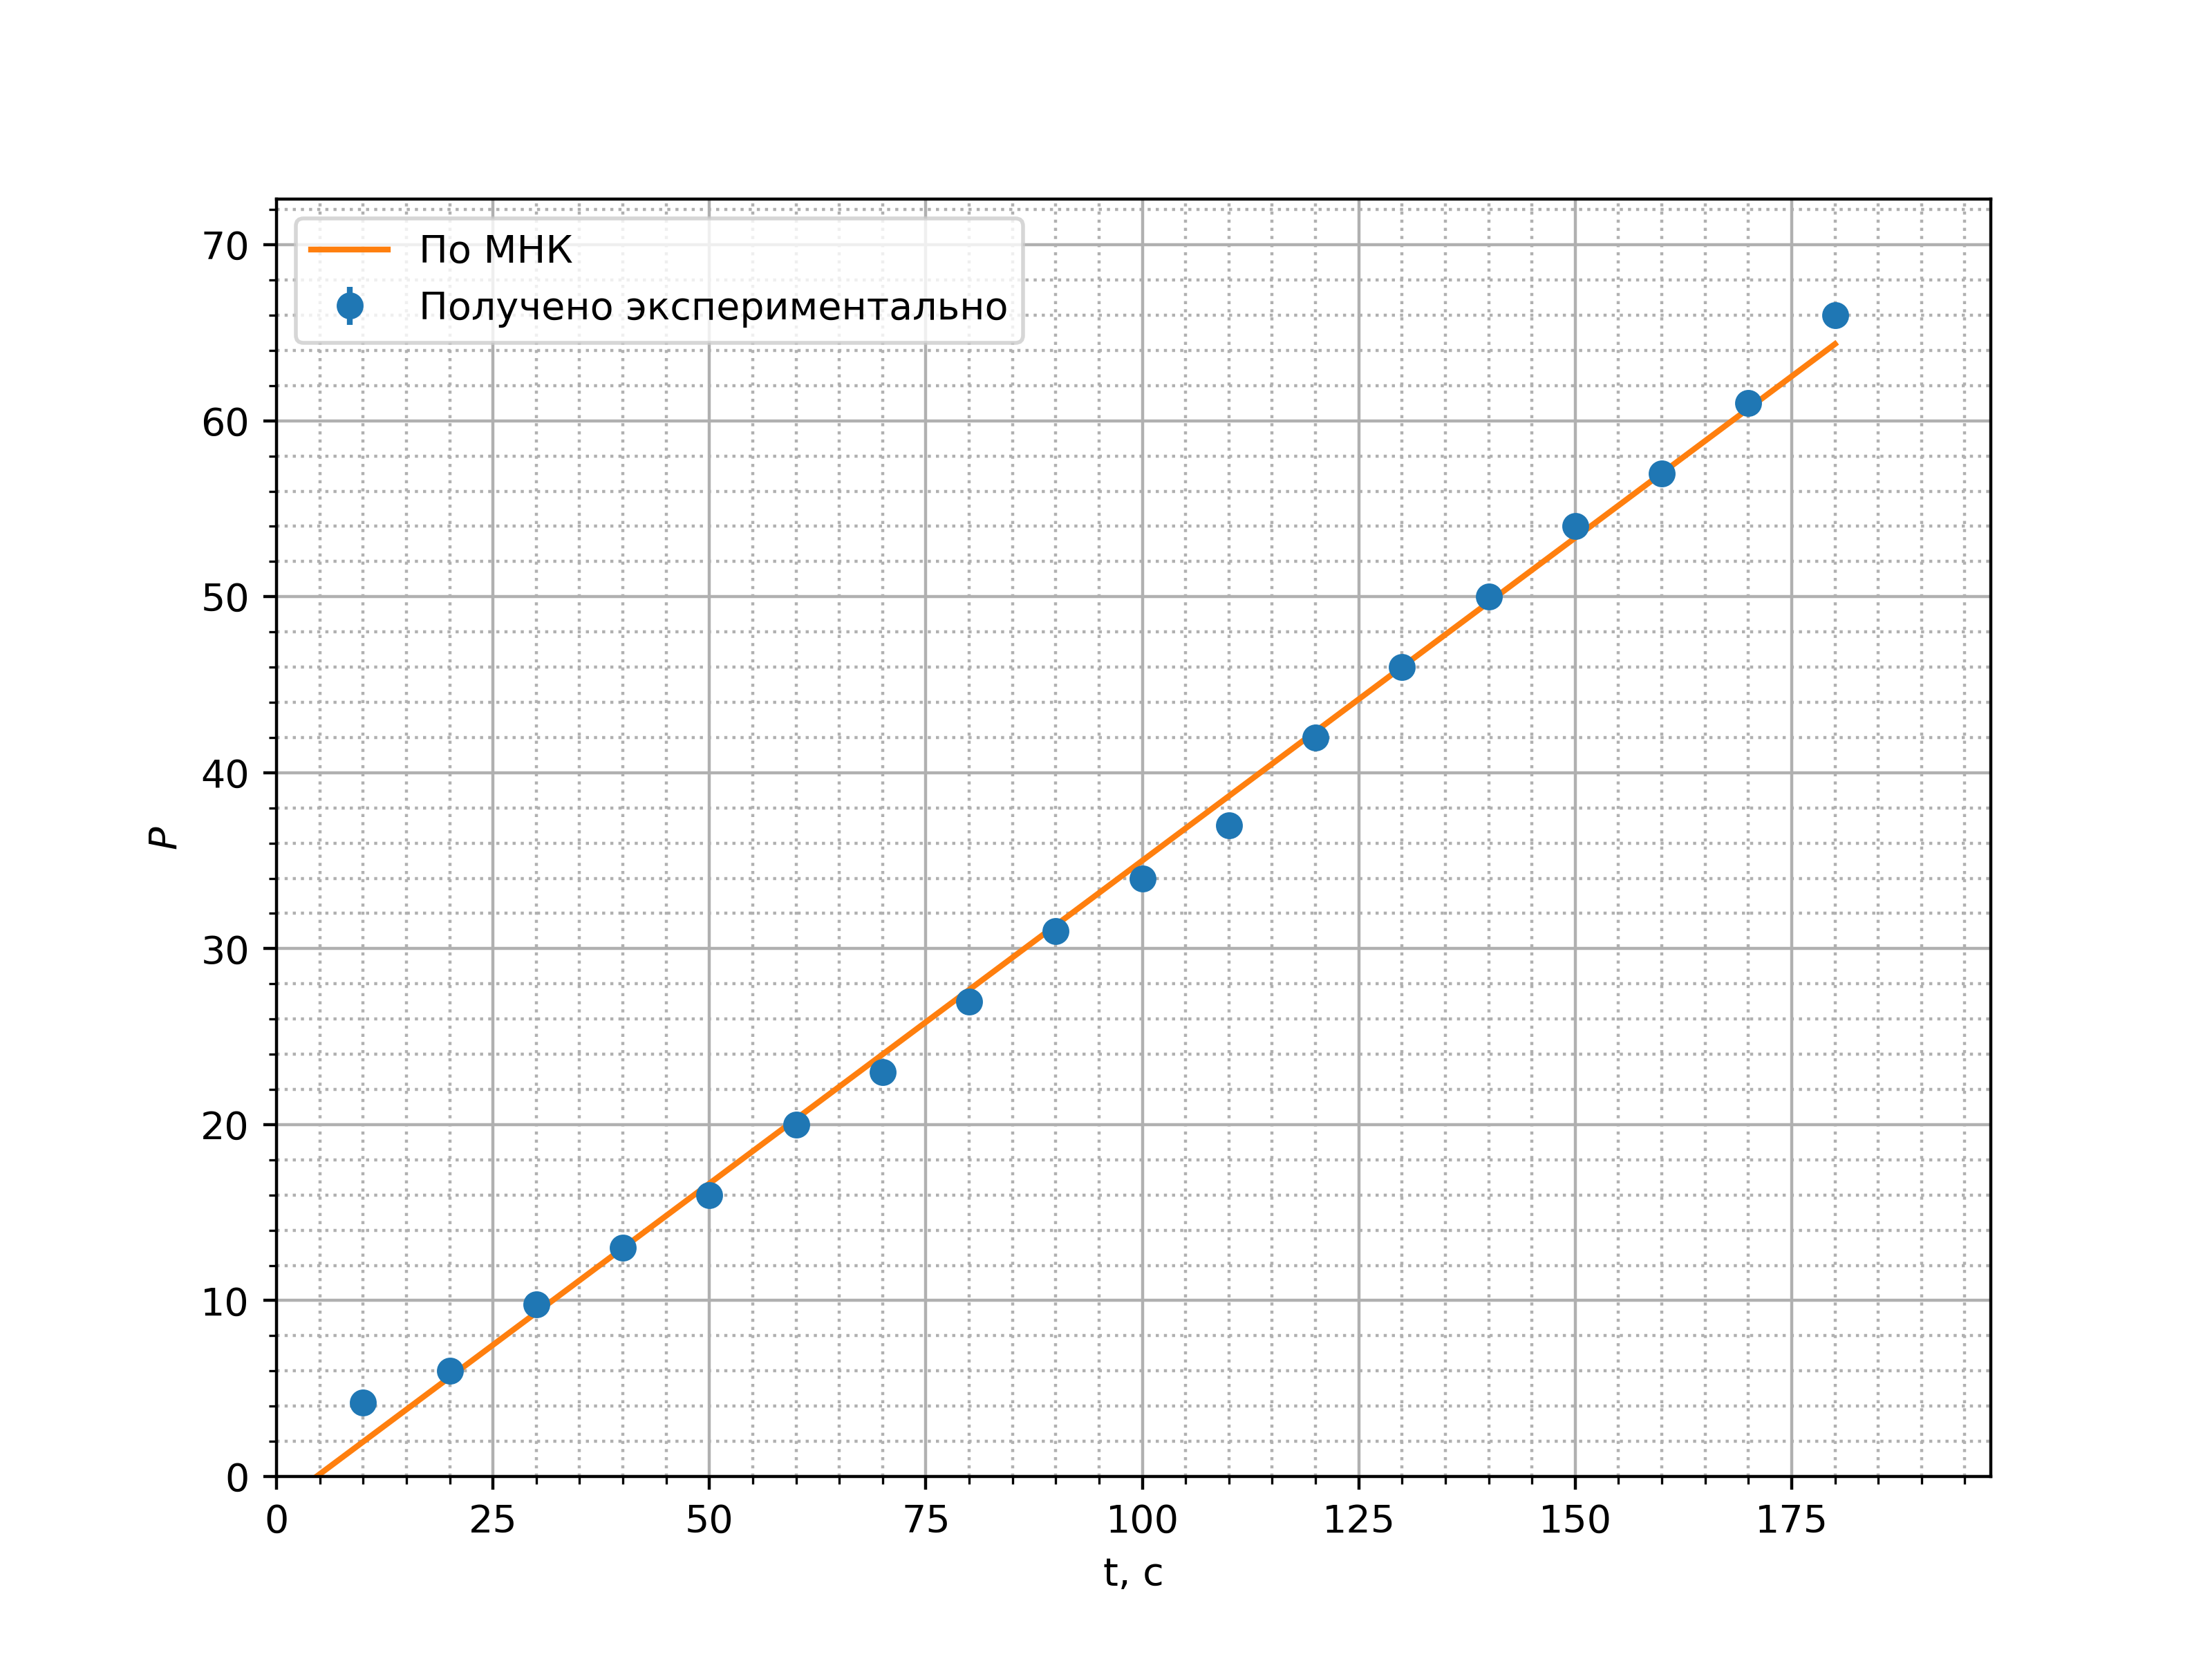
\includegraphics[width=0.5\textwidth]{diagram_3.png}}
    \hfill
    \subfloat[Ухудшение вакуума 2]{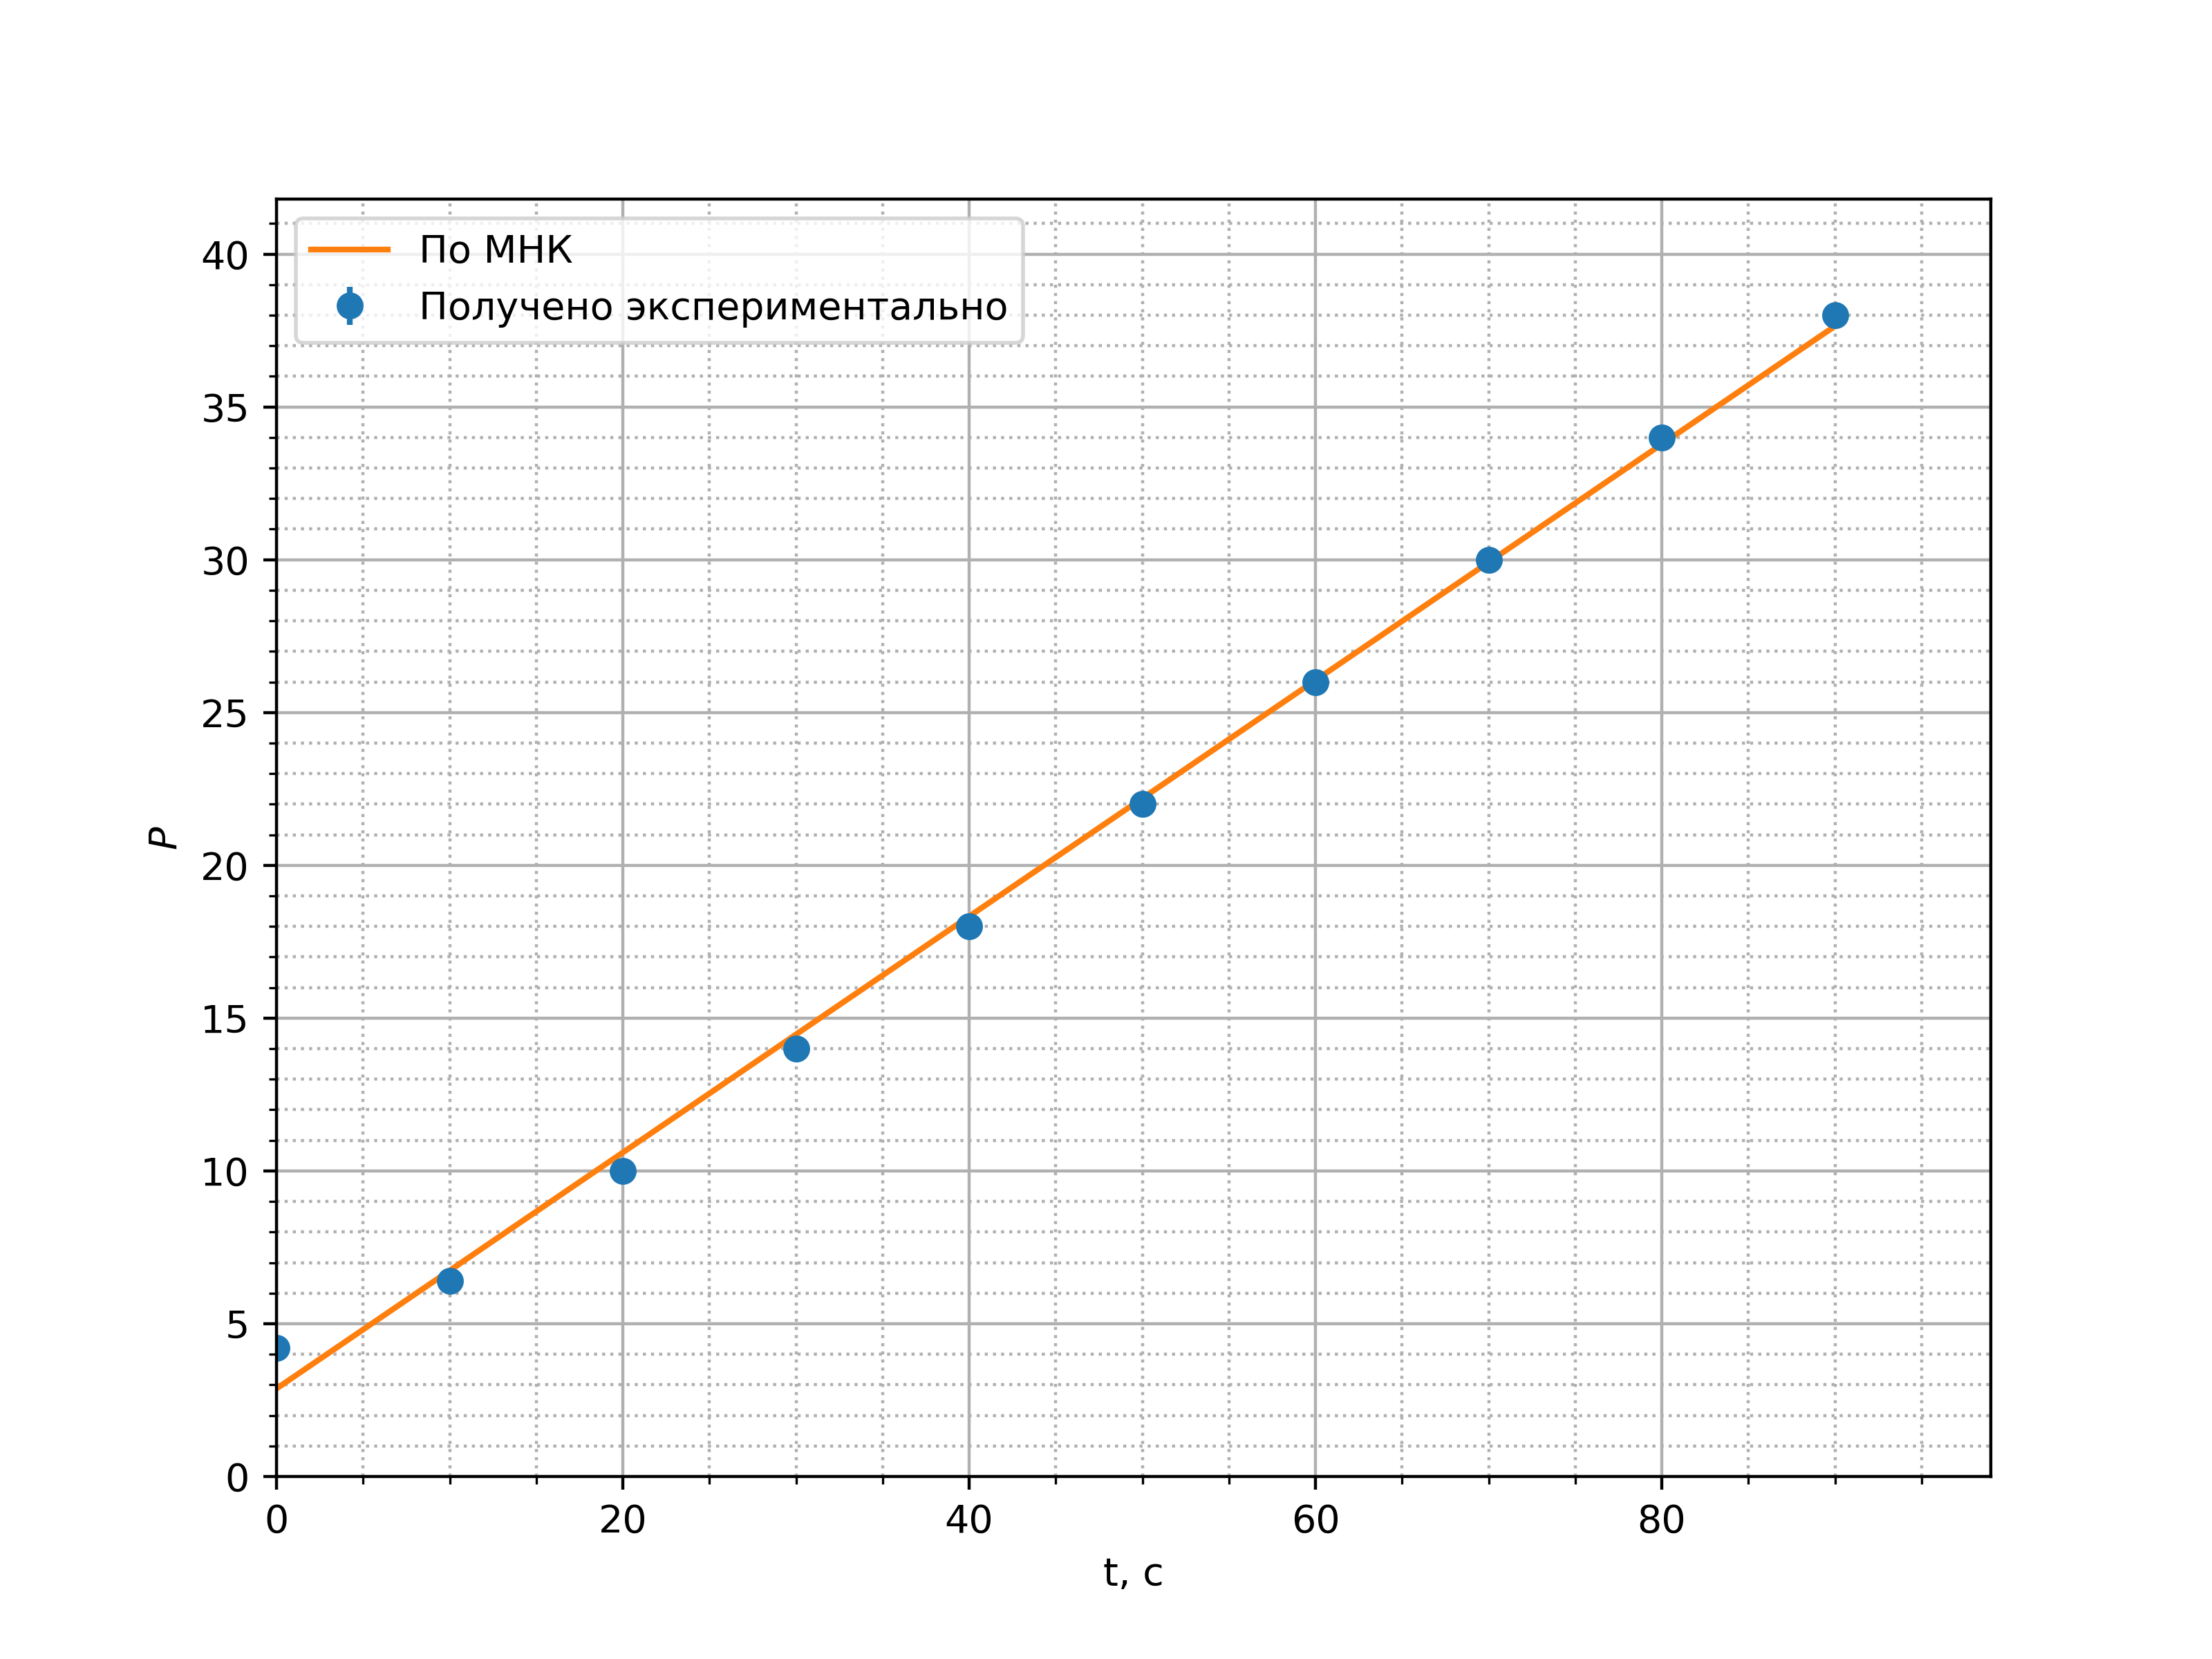
\includegraphics[width=0.5\textwidth]{diagram2_3.png}}
    \caption{Результаты экспериментов}
    \label{wawa2}
\end{figure}

Получаем:
$$ k = \frac{k_1 + k_2}{2} = \frac{0.386 + 0.366}{2} = 0.376 \Rightarrow \boxed{Q_\x{н} = k V_\x{вв} = 443.7\pm4.1 \; \frac{\x{Торр}\cdot\x{см}^3}{\x{с}}}$$

$$\sigma_Q = Q_\x{н} \sqrt{\varepsilon^2_k + \varepsilon^2_V} = 4.1 \; \frac{\x{Торр}\cdot\x{см}^3}{\x{с}}$$
$$\varepsilon_{k_1} \approx \varepsilon_{k_2} = \varepsilon_k = \sqrt{(\sigma_k^\x{случ})^2+(\sigma_k^\x{сист})^2}/k = \sqrt{0.004^2 + 0.008^2}/0.366 = 0.008 $$
$$\varepsilon_V = 6/1180 = 0.005$$

\subsection*{Оценка пропускной способности трубы}

$$d \sim 10^{-2} \; \x{м}, \qquad L\sim 1 \; \x{м}, \qquad \sqrt{\frac{RT}{\mu}} \sim 500 \frac{\x{м}}{\x{с}}$$
По формуле (\ref{eq6}), получаем:
$$\boxed{U_\x{тр} \sim 1000 \; \x{см}^3/\x{c}}$$

\subsection*{Расчёт производительности насоса}
\[
  \begin{cases}
    P_\x{пр} W = Q_1 \\
    P_\x{уст} W = Q_1 + d(PV)_\x{капилл}/{dt}
  \end{cases}
\xLongrightarrow[\x{формула (\ref{eq55})}]{} \boxed{W = \frac{4}{3}r^3\sqrt{\frac{2 \pi R T}{\mu}}\frac{P_\x{фв}}{L(P_\x{уст} - P_\x{пр})} \approx 22.15  \; \frac{\x{Торр}\cdot\x{см}^3}{\x{с}}} \]
$$ r = d/2 = 0.4 \; \x{см} \qquad L = 10.8 \; \x{см}$$
\section*{Обсуждение результатов}

В результате проделанной работы были получены значения объёмов форвакуумнойи высоковакуммной частей установки:
\begin{itemize}
    \item $V_\text{ФВ} = (2073\pm4)~\text{см}^3, \; \varepsilon_{V_\text{ФВ}} = 0.01$
    \item $V_\text{ВВ} = (1180\pm6)~\text{см}^3, \; \varepsilon_{V_\text{ВВ}} = 0.01$
\end{itemize}

Также была рассчитана скорость откачки высоковакуумным насосом:

$$W = 218.3\pm7.1  \; \frac{\x{см}^3}{c}, \; \varepsilon_W = 0.03$$

Оценено количество газа, поступающего из насоса назад в высоковакуумную часть:

$$Q_\x{н} = 443.7\pm4.1 \; \frac{\x{Торр}\cdot\x{см}^3}{\x{с}}, \; \varepsilon_{Q_\text{н}} = 0.01$$

\section*{Выводы}

В ходе данной работы:

\begin{itemize}
    \item измерены объёмы форвакуумной и высоковакуумной частей установки;
    \item получен высокий вакуум
    \item определены скорости откачки системы в стационарном режиме по ухудшению и улучшению вакуума;
    \item проверены теоретические зависимости, связанные с течением газа:
    \item проверено несколько методик по измерению производительности высоковакуумного насоса:
    \item измерено значение производительности насоса с точностью $\varepsilon = 0.03$.
\end{itemize}

\end{document}